\section{Authoring-Oriented Design Space}

We translate existing descriptive abstractions of composite visualizations
into an authoring-oriented design space. This process combines two sources of
insight. First, we conducted a study with visualization experts to establish
the granularity and perceptual organization of composable chart blocks.
Second, building on prior composition models, we operationalized composition
in terms of data and spatial relationships and examined how these
relationships are realized across coordinate systems. Together, these
analyses define the units, relationships, and spatial structures that form the
conceptual basis of {\system}.

\subsection{From Descriptive to Authoring-Oriented}

Prior work~\cite{javed2012exploring,Composite,vaid} provides descriptive
abstractions for characterizing existing composite visualizations, including
composition types such as layering, concatenation, faceting, and
nesting~\cite{vaid}. Authoring, however, requires operationalizing these
abstractions to support the construction of new compositions. This shift
raises three questions that are largely implicit in existing design spaces:
what units should be composed, what data relationships enable their
composition, and how composition is realized across coordinate systems.

\textbf{Chart blocks.}
An authoring system requires concrete and manageable units of composition.
Existing vocabularies commonly describe views using coarse chart types, but
such types may encompass structurally distinct idioms. For example, grouped,
stacked, normalized stacked, and diverging stacked bar charts differ in their
visual structures and data requirements. Conversely, treating every minor
visual variation as a separate unit would unnecessarily fragment the design
space. An authoring-oriented design space must therefore establish a block
granularity that captures consequential structural differences while
abstracting away stylistic variations.

\textbf{Data dimensions.}
Chart idioms require different combinations of categorical, quantitative,
temporal, geographic, hierarchical, or relational dimensions. Composition
further introduces relationships among the data used by different blocks,
such as shared positional dimensions for layering, partitioning dimensions
for faceting, or correspondence keys for nesting. These data requirements and
cross-block relationships must be made explicit to guide how blocks can be composed.

\textbf{Coordinate systems.}
Existing composition models are largely grounded in two-dimensional Cartesian
space. Authoring across other coordinate systems requires
these relationships to be interpreted through different spatial dimensions.
For example, polar coordinates support angular and radial arrangements,
whereas geographic coordinates introduce projection- and
reference-dependent placement. An authoring-oriented design space must
therefore distinguish abstract composition types from their
coordinate-specific spatial realizations.

Together, these considerations extend existing descriptive abstractions into
an authoring-oriented design space organized around composable chart blocks,
their data relationships, and their spatial realization across coordinate
systems.

\subsection{Expert Study of Composable Chart Blocks}
Chart blocks define the units that an authoring system can instantiate,
manipulate, and compose. We establish their granularity and organization
through an expert-grounded analysis of the VAID corpus~\cite{vaid}, which
contains 442 composite visualizations.

\textbf{Expert involvement.}
We recruited 6 visualization experts (E1--E6), including 4 academic
researchers (E1--E4) and 2 industry practitioners (E5, E6). All experts had
more than 5 years of professional or research experience in visualization
and had designed and implemented composite visualizations in the development
of visual analytics systems or related applications. In addition, E1 and E3
had prior experience conducting visualization surveys and had systematically
studied the classification, application contexts, and visual forms of
visualizations. Their complementary expertise in visualization research,
system development, and practical design informed both the decomposition of
composite visualizations into chart blocks and the subsequent organization of
these blocks into perceptually meaningful families.

\textbf{Block granularity.}
The experts independently decomposed 100 representative visualizations sampled
from the corpus into constituent chart units. Without a predefined taxonomy,
they identified units that they considered visually coherent and meaningful
to construct or manipulate independently. We compared their decompositions to
identify recurring block boundaries, obtaining substantial inter-rater
agreement (Fleiss' $\kappa=0.74$). Based on these judgments, we distinguish
blocks when their structural differences affect data requirements, encoding
behavior, or subsequent composition. For example, grouped, stacked,
normalized stacked, and diverging stacked bar charts are treated as distinct
blocks because they organize marks and data differently, whereas minor
stylistic variations do not generally define separate blocks.

\textbf{Perceptual organization into families.}
The experts then organized the resulting blocks into chart families through
an association-driven grouping task. Rather than asking them to derive a
formal taxonomy, we asked which blocks they would expect to find under the
same broad category in an authoring tool and which ones they would regard as
design alternatives. We converted their co-grouping judgments into pairwise
similarities and used hierarchical clustering and majority agreement to
derive candidate families, while retaining their qualitative rationales to
interpret relationships within each family. This procedure prioritizes how
authors recognize and search for chart designs rather than how developers
might organize them based solely on implementation similarity.
The experts' rationales revealed three recurring factors that shape family
organization and the presentation of alternatives:

\emph{Coordinate system.}
A change of coordinate system can produce chart idioms that are structurally
related but perceptually distinct. For example, icicle plots and sunburst
charts represent similar hierarchical structures in Cartesian and polar
coordinates, respectively. Most experts initially identified them as distinct
chart types, whereas E1 and E3, who had prior experience developing chart
classifications, explicitly associated them as coordinate-system alternatives.
This suggests that an authoring tool should preserve both idioms as
recognizable options while making their structural relationship accessible.

\emph{Data dimensionality.}
Differences in data requirements frequently define alternatives within a
family. This consideration was especially prominent for bar charts: experts
associated grouped and stacked variants with the basic bar chart while
recognizing that they introduce additional data dimensions and corresponding
mark organizations. Such variants should therefore remain connected within a
family without being collapsed into a single block.

\emph{Visual style.}
Stylistic differences can also affect how users identify and retrieve a chart.
E1 and E3 regarded a step line chart primarily as a variant of a line chart.
E4 agreed with this relationship but emphasized that step lines are often
sought as a distinct, domain-specific idiom, for example in financial
visualization, an author with such a use case may search directly for a step
line chart rather than derive it as a style variation of a line chart. We
therefore use family relationships to connect stylistic alternatives while
retaining directly recognizable blocks where appropriate.


\textbf{Block specification.}
Each block is specified by its chart idiom, data requirements, encoding
channels, and supported coordinate systems. Drawing on the visualization
primitives and encoding abstractions of D3.js~\cite{bostock2011d3} and
Vega-Lite~\cite{satyanarayan2016vega}, we annotate the visual channels supported by each
block, including position, length, color, size, shape, and angle. The chart
idiom describes the block's visual structure, such as a grouped bar chart,
line chart, scatterplot, or area chart. Its data requirements specify the
number and semantic roles of the required dimensions, with each dimension
annotated by data type, such as categorical, quantitative, temporal,
geographic, hierarchical, or relational. Coordinate support identifies the
spatial dimensions and coordinate systems through which these data dimensions
are visually encoded.



\subsection{Dimension-Aware Composition}
Existing composition types have been derived primarily from visualizations in
two-dimensional Cartesian space. We therefore first operationalize these
types in terms of their relationships along the $x$ and $y$ dimensions. In
particular, we require a composition to couple blocks in both data space and
display space: the blocks must have an operator-specific relationship between
their data dimensions or entities, and this relationship must be reflected by
their spatial arrangement. Blocks that are merely aligned or placed adjacent
without a data-space relationship are treated as layout arrangements, whereas
blocks that use related data but are positioned independently remain separate
charts. Following VAID~\cite{vaid}, we consider four composition types:
layering, concatenation, faceting, and nesting.

\textbf{Layering} places multiple blocks in the same plotting region and couples them
along both coordinate dimensions. In Cartesian space, layered blocks share
both the $x$ and $y$ axes, including compatible dimensions, scales, and spatial
positions. For example, a line chart and an area chart can be layered when
their horizontal and vertical encodings can be expressed in a common
coordinate space.

\textbf{Concatenation} places blocks in adjacent plotting regions while coupling them
along one coordinate dimension. Horizontally concatenated blocks share and
align their $y$ axis while occupying separate regions along $x$; vertically
concatenated blocks share and align their $x$ axis while occupying separate
regions along $y$. Thus, adjacency alone does not constitute concatenation:
blocks placed side by side without a shared and spatially aligned axis are
treated as a layout arrangement.

\textbf{Faceting} partitions data by one or more dimensions and instantiates a common
chart block for each partition. The instances preserve the same chart idiom
and encoding structure and are systematically positioned according to the
faceting dimensions. Faceting therefore couples instances through both a
shared visualization specification and a spatial arrangement determined by
the partitioning dimension.

\textbf{Nesting} associates child-block instances with a collection of
repeated internal elements in a parent block. Nesting applies the same child-block specification to each
eligible parent element. These elements may be data-driven marks, such as
points in a scatterplot, or repeated structural components, such as axes in a
parallel coordinates plot. For each parent element, the system instantiates a
child block and establishes its data-space relationship through a shared key,
a filtering condition, or a hierarchical correspondence. The child instance
is then positioned relative to the spatial reference of the corresponding
element, such as its position, extent, or boundary.

Under this definition, layering shares two coordinate dimensions,
concatenation shares one, faceting derives repeated blocks from a partitioning
dimension, and nesting establishes a parent--child correspondence. In each
case, composition is distinguished from general layout by the joint presence
of data-space and display-space relationships.


\subsection{Extending Composition Across Coordinate Systems}

The preceding definitions operationalize composition in Cartesian space. We
further consider how these composition types extend to other coordinate
systems represented on a two-dimensional plane. 

\textbf{Coordinate-system requirements.}
Layering and concatenation require the participating blocks to use the same
coordinate system, since they share two and one of its spatial dimensions,
respectively. Nesting does not impose this requirement: the parent and child
may use different coordinate systems because their relationship is
established through a parent anchor. Faceting is similarly independent of the
coordinate systems of the repeated blocks, it introduces an
outer coordinate system that determines how the block instances are arranged.

\begin{figure}[h]
  \centering
  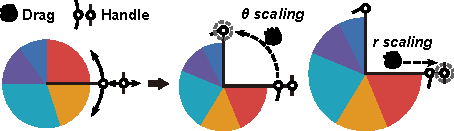
\includegraphics[width=\columnwidth]{figs/polar_scale.pdf}
  \caption{Interactive polar scale control. Our design enables independent 
scaling of angular ($\theta$) and radial ($r$) dimensions. Left to right: 
origin scale; adjust angular range via 
$\theta$ handle; modify radial extent via $r$ handle.}
  \label{polar_scale}
\end{figure}


\textbf{Polar coordinates.}
Polar coordinates provide an angular dimension $\theta$ and a radial
dimension $r$. Of particular interest is concatenation, which has two
coordinate-specific forms: angular concatenation partitions $\theta$ while
sharing $r$, producing adjacent sectors, whereas radial concatenation
partitions $r$ while sharing $\theta$, producing concentric rings. The same
dimensions also define the arrangement of a polar facet. 
Notably, angular concatenation may assign different angular sectors to
different chart blocks rather than requiring each block to span the full
$0^\circ$--$360^\circ$ range. For example, a pie chart and a polar dot plot
can each occupy one half of the polar space while sharing the radial
dimension (\autoref{fig:drag-drop}.B2). However, 
traditional polar visualizations assume a fixed full-circle range. To address 
this, we introduce interactive scaling controls (\autoref{polar_scale}) that enable dynamic adjustment 
of both $\theta$ range and $r$ scale through direct manipulation handles on 
the axes, providing more flexible control over the polar coordinate space.


\textbf{Geographic coordinates.}
Geographic coordinates use longitude and latitude to specify locations rather
than allocate independent chart regions. We therefore support layering in a
shared geographic reference and nesting through geographic anchors, such as
points or regions. Concatenation and faceting are not defined directly over
geographic coordinates because they require additional assumptions about
projections, boundaries, or regional partitions.

\textbf{Coordinate-free layouts.}
Coordinate-free layouts position elements either through layout algorithms,
such as tree or force-directed layouts, or through positions explicitly
specified by the user. Although these layouts assign positions to elements,
the positions do not constitute shared spatial dimensions with explicit
coordinate semantics. They therefore do not directly support the dimension
sharing required by layering and concatenation. Coordinate-free blocks may
nevertheless participate in nesting through element-level anchors or appear
within a facet whose arrangement is defined by an external coordinate system.